\newcommand{\mola}[4]%Quanto menor for o valor 3,4 e 5 dado à função mais comprimida estará a mola%
{
%------------------------------------------------------------Pontos Importantes------------------------------------------------------------%
\coordinate (bola1) at (0,{#1});
\coordinate (bola2) at (0,{#2}); 
\coordinate (bola3) at (0,-4);
\coordinate (bola4) at (0,-8);
\coordinate (reticencias) at (0,-6);
%-------------------------------------------------------------Desenhar as Molas------------------------------------------------------------%
\tikzstyle{spring}=[thick,decorate,decoration={aspect=.5, segment length=#3, amplitude=2.5mm,coil}]
\draw [spring] (bola2) -- (bola1);
\draw [spring] (bola3) -- (bola2);
\tikzstyle{spring}=[thick,decorate,decoration={aspect=.5, segment length=#4, amplitude=2.5mm,coil}]
\draw [spring] (bola4) -- (bola3);
%-------------------------------------------------------------Desenhar as Bolas------------------------------------------------------------%
\shade [ball color =white] (bola1) circle (.5) node[draw=none,inner sep = 0,scale=2,text=black]{};
\shade [ball color =white] (bola2) circle (.5) node[draw=none,inner sep = 0,scale=2,text=black]{};
\shade [ball color =white] (bola3) circle (.5) node[draw=none,inner sep = 0,scale=2,text=black]{};
\shade [ball color =white] (bola4) circle (.5) node[draw=none,inner sep = 0,scale=2,text=black]{};
%----------------------------------------------------------Desenhar as Reticências--------------------------------------------------------%
\node[rectangle,fill=white, minimum width = 2cm, minimum height = 1.1cm] (r) at (reticencias) {};
\draw (reticencias) node[ultra thick,scale=1,yshift=.05cm]{$\rotatebox{90}{$\cdots$}$} ;
}
\begin{minipage}{0.22\colwidth}
\resizebox{.2\colwidth}{!}{
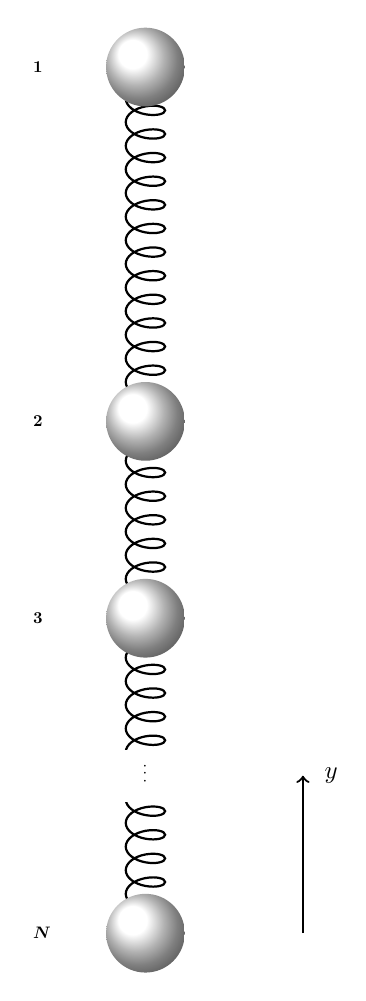
\begin{tikzpicture}[scale=1, every node/.style={scale=.6}]
\mola{3}{-1.5}{3mm}{3mm}
\node[anchor=west] at (-1.5,3) {\textbf{\boldmath$1$}};
\node[anchor=west] at (-1.5,-1.5) {\textbf{\boldmath$2$}};
\node[anchor=west] at (-1.5,-4) {\textbf{\boldmath$3$}};
\node[anchor=west] at (-1.5,-8) {\textbf{\boldmath$N$}};
\draw[thick,->] (2,-8) -- (2,-6) node[draw=none,inner sep = 0,scale=1.5,xshift=.4cm,text=black]{$y$};
\end{tikzpicture}}
\end{minipage}
\begin{minipage}{0.7\colwidth}
Descrevemos uma mola ideal com constante elástica $K$, comprimento natural $L$ e massa $M$ como um sistema de $N$ massas $m=M/N$ ligadas sequencialmente por $N-1$ molas ideais com comprimento natural $l=L/(N-1)$ e constante elástica $k=K(N-1)$.\\[1ex]   
%\begin{align*}
%  l&=L/(N-1)&&\rightarrow\text{Comprimento de cada segmento}\\
%  k&=K(N-1)&& \rightarrow\text{Constante elástica de cada segmento}\\
%  m&=M/N    &&\rightarrow\text{Massa de cada partícula}
%\end{align*}
Em equilíbrio estático, as posições das várias massas são dadas por:
\begin{equation*}
  %y_i^0=y_0^0-i\left[l+\left(N-\frac{i+1}{2}\right)\frac{mg}{k}\right],\quad i>0
  y_i^0=y_1^0-(i-1)\left[l+\left(N-\frac{i}{2}\right)\frac{mg}{k}\right],
  \quad i>1
\end{equation*}
A partir do instante em que se solta a massa na extremidade superior da mola, as acelerações das várias massas são dadas por ($x_i(t)=y_i(t)-y_i^0$, $\ddot x_i=\ddot y_i$, $\omega^2=k/m$):
  \begin{align*}
    %\ddot x_0 &=-Ng+\omega^2(x_1-x_0)\\
    \ddot x_1 &=-Ng-\omega^2(x_1-x_2)\\
    \ddot x_i &= \omega^2(x_{i-1}-2x_i+x_{i+1}),\qquad i=2, \ldots, N-1\\
    %\ddot x_{N-1} &=\omega^2(x_{N-2}-x_{N-1})
    \ddot x_{N} &=\omega^2(x_{N-1}-x_{N})
  \end{align*}
\end{minipage}\\[1cm]
Este sistema de equações, com o estado inicial $x_i=0$, $\dot x_i=0$, foi resolvido em Python/Numpy \cite{harris2020array}, usando a função
\texttt{solve\_ivp} da biblioteca SciPy \cite{2020SciPy-NMeth}.
